\documentclass[conference]{IEEEtran}
\IEEEoverridecommandlockouts

\usepackage{cite}
\usepackage{amsmath,amssymb,amsfonts}
\usepackage{algorithmic}
\usepackage{graphicx}
\usepackage{textcomp}
\usepackage{xcolor}
\usepackage{booktabs}
\usepackage{array}
\usepackage{url}
\def\BibTeX{{\rm B\kern-.05em{\sc i\kern-.025em b}\kern-.08em
    T\kern-.1667em\lower.7ex\hbox{E}\kern-.125emX}}

\begin{document}

% NOTE: the assignment brief says the report must include the student number
% in the title section and must NOT include name, surname or other identifying
% information. Author block below therefore carries the student number only.

\title{Ensemble Learning for Network Attack Classification on the UNSW-NB15 Dataset
\thanks{Code available at: https://github.com/T-Bone183/ML-Project4-26690071}}

\author{
\IEEEauthorblockN{26690071}
\IEEEauthorblockA{
\textit{Department of Computer Science} \\
\textit{Stellenbosch University} \\
Stellenbosch, South Africa \\
26690071@sun.ac.za}
}

\maketitle

\begin{abstract} %[DONE]
% rubric: Abstract (4)
The modified UNSW-NB15 dataset poses a severely imbalanced, ten-class network-attack classification
problem. Earlier work on it compared a $k$-nearest-neighbours classifier with a single classification
tree and found the tree to be the better model, achieving a macro-averaged $F_1$ score of $0.580$, with
the rare attack classes being its main weakness. This report investigates whether that result can be
improved, either by changing the underlying tree algorithm or by combining trees into an ensemble,
through a $2\times2$ comparison of two base learners, CART and C4.5, each as a single tree and
as a bagged random forest. The C4.5 models were implemented from scratch, since no suitable library was
available. All four were tuned by grid search on a held-out tuning set and evaluated by macro-averaged
$F_1$ under stratified five-fold cross-validation, reusing the earlier work's data split
so that the results remain comparable. Ensembling improved both base learners, but only
by a small margin of around $0.008$ in macro-$F_1$. The
best model, the CART random forest, achieved a score of $0.588$. The choice of base learner did not make a significant
difference since CART and C4.5 were statistically indistinguishable as both trees and forests, and C4.5's
gain-ratio criterion did not offer an advantage. Most of the remaining errors fall on a small number of rare attack classes that overlap heavily with others and
are difficult to distinguish, so the limit on performance points to the data itself rather than the choice of
tree-based model.
\end{abstract}

\section{Introduction} %[DONE]
% rubric: Introduction (8)

Differentiating between normal network traffic and specific categories of attack is a core task
in intrusion detection. The nature of the data itself makes this a challenging task since
real traffic is dominated
by a few common classes, leaving the rarest attacks represented by only a handful of examples.
Earlier work on the modified UNSW-NB15 dataset referred to in this report compared a $k$-nearest-neighbours
classifier with a single classification tree, and found the tree to be the stronger model, achieving
a macro-averaged $F_1$ score of $0.580$. Its main weakness was the minority attack classes, which it
classified poorly.

This report investigates whether the results can be improved in two ways. The first is by changing 
the base learner: the previous tree used the CART algorithm, while C4.5 allows multi-way categorical 
splits and uses the gain-ratio criterion, both of which may be better suited to the high-cardinality 
categorical features in this dataset. The second is by increasing model complexity through ensembling. 
A random forest combines multiple decorrelated trees to reduce variance and potentially improve 
predictive performance. Combining these two approaches gives four models in a $2\times2$ design: 
CART and C4.5, each implemented as both a single tree and a random forest. This allows the effects 
of the choice of base learner and ensembling to be examined separately. The main questions are 
whether C4.5 outperforms CART, and whether using a random forest improves the performance of 
either algorithm.

A random forest was chosen as the ensemble rather than a boosting method for two reasons. First, it
extends the existing single-tree baseline without changing the learning algorithm, which keeps the
comparison simple. Second, it is more robust to inherently ambiguous data: boosting repeatedly
up-weights the instances it misclassifies, so when classes overlap heavily in feature space it
fixates on the ambiguous boundary cases that cannot be classified reliably, and is for this reason
less robust than bagging~\cite{dietterich2000}. As the results will show, the attack classes in this
dataset overlap substantially, making bagging the safer choice. Because no established library implements C4.5, the
two C4.5 models were written from scratch. This also made it possible to test the gain-ratio
criterion directly --- something the earlier CART tree could not do, as the \texttt{scikit-learn}
library it used does not offer gain ratio.

All four models were tuned and evaluated on the same stratified data split and macro-$F_1$ protocol
as the earlier work, so that the new results sit directly alongside it. The remainder of the report
is organised as follows. Section~II provides background on the dataset, the two tree algorithms, and
ensemble learning. Section~III describes the implementation and Section~IV the empirical procedure.
Section~V presents and discusses the results, and Section~VI concludes.

\section{Background} %[DONE]
% rubric: Background (24)
%Add a quick background on the dataset with the biggest glaring issue being the
%target class imbalance as well as the missing values (not an issue)

%[DONE]
This study focusses on a supervised multi-class classification problem: predicting the
category of a network traffic record from a modified version of the well-known UNSW-NB15 
intrusion detection dataset \cite{moustafa2015unsw}. 

The approximately $257{,}000$
observations have $42$ predictive features --- a mixture of both numeric 
and nominal fields --- and are each labelled with one of ten target
classes, nine of which are attack categories with the remaining one constituting normal traffic.
Three properties of the data are relevant to the modelling that follows.
Firstly, the target distribution is highly imbalanced:
the largest classes contain tens of thousands of observations while the rarest class,
\texttt{Worms}, contains only $174$. Secondly, the
\texttt{service} feature has $54.8\%$ of its records missing. Thirdly, several nominal
features have a high cardinality, most notably \texttt{proto} with $133$ different
categories.

\subsection{Baseline Models: k-Nearest Neighbours and Classification Trees} %[DONE]
% restate the Assignment 2 models being compared against

Previous work on this dataset \cite{a2} explored two baseline classifiers against which
the present work is compared. These were a $k$-nearest neighbours (kNN) classifier and a single
classification tree.
Both were tuned and evaluated in an identical manner, which
is reused here so that the comparison between all of the models remains fair.
A tuning set of
$50{,}000$ observations is held separate from a training/test set of the remaining
$\approx\!207{,}000$ observations, with hyperparameters selected by grid search using
five-fold cross-validation, and performance evaluated using the
\emph{macro-averaged $F_1$ score}. The definition and justification for using
the macro-$F_1$ metric is discussed further in the Performance Metric section.

Under this protocol the classification tree outperformed kNN with a macro-$F_1$ of
$0.580$ against $0.548$. 

The tree’s advantage comes from how it constructs decision regions: it splits on one
feature at a time, producing axis-aligned partitions that can approximate non-linear 
boundaries through multiple recursive splits. This allows it to work in the presence of both
numeric and nominal features without forcing them into a single global distance measure, 
as kNN does. Numeric features are handled through threshold splits, while nominal 
features can be partitioned into subsets of categories, so the model does not need a 
shared scale or a common notion of closeness across all attributes.

The tree is also more robust under severe class imbalance. For kNN, the \(k\) nearest 
neighbours of an unseen minority-class observation are likely to be dominated by
majority-class instances, even when making use of distance weighting. In this 
manner neighbourhood voting can overwhelm the rare classes.
A tree, on the other hand, can keep splitting until it isolates leaves that 
are comparatively pure in the minority class.

It is worth noting that the one-hot encoding of high-cardinality categorical features such as 
\texttt{proto} is \emph{not} the main hindrance. As argued in the prior study \cite{a2}, 
under the distance metric used, the one-hot block for a categorical variable always contributes 
either zero (when categories match) or a fixed constant (when they mismatch). The expansion 
therefore behaves more like a single binary term than like many independent 
dimensions when considering the similarity measure. The tree is thus the stronger of the two 
baselines and lays the foundation of this work: given that a tree-based model is the best performer so far, 
\emph{can performance be improved by using a different tree, or by aggregating trees into 
an ensemble?}

\subsection{Decision tree induction and limitations of the Assignment 2 Implementation} %[DONE]
% CART vs C4.5 / scikit-learn limitations motivating the new approach

%Briefly discuss what was implemented and how (preprocessing necessary), then discuss
%the limitations of cart (no gain ratio and only binary splits - also link between
%these two is worth noting)
The baseline tree was implemented with scikit-learn's \texttt{DecisionTreeClassifier},
which makes use of the CART induction algorithm \cite{breiman1984cart}. CART induces a tree
by recursive \emph{binary} partitioning. Starting at the root, it greedily selects, over all
features and possible split points, the binary split that most reduces node impurity as
measured by the Gini index, divides the observations into the two resulting child nodes,
and repeats this recursively until a stopping criterion is met, at which point each leaf
predicts the majority class of the training observations it contains. Thereafter overfitting is
limited by applying cost-complexity pruning.
This induction strategy imposes several
limitations that a C4.5 tree \cite{quinlan1993c45} is specifically designed to address.
Firstly, CART produces only \emph{binary} splits and does not support multi-way
categorical splitting. As a result a high-cardinality nominal feature such as \texttt{proto} must
therefore be one-hot encoded into $133$ indicator columns before fitting. Secondly,
its split criterion is restricted to the Gini index or entropy (plain information gain),
with no support for \emph{gain ratio}. This is the criterion native to C4.5, introduced to
counteract the bias of information gain toward high-cardinality features. 
These two
limitations are linked: gain ratio exists precisely to take into account the many-valued-feature
bias that multi-way splitting introduces, so an algorithm that does not make use of multi-way splits
avoids that bias by a different route (such as CART only allowing for binary splits). 
Finally, CART requires missing values to be resolved before
fitting, and cannot perform C4.5's native treatment of distributing an instance with a
missing split value across branches in proportion to their frequency. Together these
points motivate extending the previous work done on this dataset by implementing a C4.5 tree 
as an alternative base learner to assess how its performance compares to the CART tree, before
moving on to the main focus of this work.

C4.5 shares CART's overall divide-and-conquer strategy --- a tree is grown top-down by
recursively selecting a split, partitioning the training observations, and recursing
until a stopping criterion is met, producing a leaf that predicts its majority class. The primary differences are
in how it splits, how it scores those splits, and how it prunes. Where CART is restricted
to binary splits, C4.5 performs \emph{multi-way} splits on nominal features, creating one
branch per category, while still splitting numeric features via a binary
threshold. 
Its split criterion is entropy-based. For a set $S$ of observations with class
proportions $p_c$ over $M$ classes, node impurity is measured by entropy (and, in CART's
case, the Gini index),
\begin{equation}
H(S) = -\sum_{c=1}^{M} p_c \log p_c,
\qquad
G(S) = 1 - \sum_{c=1}^{M} p_c^2 ,
\end{equation}
and a candidate split partitioning $S$ into subsets $\{S_j\}$ yields the \emph{information
gain}
\begin{equation}
\mathrm{IG}(S) = H(S) - \sum_j \frac{|S_j|}{|S|}\, H(S_j),
\end{equation}
the reduction in entropy achieved by the split. Splits under consideration are scored by
information gain or, as mentioned earlier, the \emph{gain ratio}. The gain ratio divides
the information gain of a split by its \emph{split information},
\begin{equation}
\mathrm{SI}(S) = -\sum_{j=1}^{k} \frac{|S_j|}{|S|} \log \frac{|S_j|}{|S|},
\end{equation}
where the split partitions the node's observations $S$ into $k$ branches
$S_1,\dots,S_k$. Note that split information has the same functional form as entropy, but is
computed using \emph{branch sizes} rather than target labels. 
It measures how widely and evenly the split distributes the observations amongst its branches,
without considering the target labels in those branches. A balanced binary split has a small
split information, whereas a split on a high-cardinality feature such as \texttt{proto},
which scatters the data across many small branches, has a large one. Dividing the
information gain by this quantity penalises splits that achieve a high gain by purely fragmenting
the data, which acts against the many-valued-feature bias noted above. 
Pruning differs as well and is an important point to note since the original
C4.5 limits overfitting through pessimistic, error-based pruning that estimates each
subtree's error from the training data alone. The implementation used here instead applies
\emph{reduced-error pruning} (REP), in which, after the tree is fully grown, subtrees are
examined bottom-up and a subtree is collapsed into a single leaf whenever doing so does not
increase the classification error on a held-out pruning subset. REP is used instead due to its
simplicity which makes it easy to implement while at the same time being
reported to achieve generalisation performance on par with
C4.5's native pruning \cite{esposito1997}. For this reason the single-tree model is referred to
throughout as \emph{C4.5 with REP}.
%???citation above should be a citation that shows how different pruning strats don't
%really offer significantly improved performance


\subsection{Ensemble Learning} %[DONE]
% chosen ensemble method, bias--variance framing

An ensemble combines the predictions of many \emph{base learners} into a single, typically more
accurate, aggregate predictor. The ensemble method used here is the \emph{random
forest} \cite{breiman2001randomforests}, a form of \emph{bagging} (bootstrap
aggregating) \cite{breiman1996bagging} which uses decision trees as base learners. 
The best way to understand the design of an ensemble is through the lens of the
bias--variance decomposition of generalisation error. 
An unpruned decision tree is a low-bias, high-variance estimator: it fits the training
data closely, due to the lack of pruning which would improve generalisation performance and is therefore
unstable, since small changes to the data can produce a very different tree. 

Bagging reduces this \emph{variance} without increasing bias
by training each tree on a bootstrap resample of the data and averaging their votes.
So long as the trees are not perfectly correlated, i.e. there is variability amongst their predictions,
the variance of the aggregate is lower than that of any single tree. 
A random forest further \emph{decorrelates} the trees by
restricting each split to a random subset of the features, which is what sets it apart
from plain bagging.

Random forests, rather than a boosting ensemble, were chosen for two reasons. The first
is due to the prior work on this dataset. Because the baseline model is already a single tree, bagging
\emph{extends the same base learner} into an ensemble, and the comparison therefore
isolates the effect of ensembling itself rather than confounding it with a change of
learning algorithm. This gives a clean $2\times2$ design: the two base learners, CART and C4.5, each evaluated
both as a single tree and as a forest --- four models in total. Comparing these models
answers two questions at once: whether C4.5 outperforms CART as a single tree, and whether
turning each base learner into a forest improves its performance.
Boosting, by contrast, fits a sequence of reweighted learners and would
alter the learning approach entirely rather than extending it. The second
reason is robustness. Boosting progressively increases the weight of the
instances it misclassifies, in order to force later learners to correct them. When
classes overlap heavily in feature space, however, the persistently misclassified
instances are the inherently ambiguous cases on the class boundaries, which cannot be
classified reliably. Boosting fixates on these and is for this reason less robust than
bagging \cite{dietterich2000}. Bagging, which resamples rather than reweights, is
comparatively unaffected, making a random forest the more defensible choice for a dataset
with the degree of class overlap seen here.

The random forest is simply a generic procedure applied on top of either base learner: it reuses
the same tree-induction algorithm, grown without pruning, and adds bootstrap resampling of
the training data, a random feature subspace at each split, and majority voting across the trees.
Given a training set of $N$ observations, each of the $B$ trees is induced on a bootstrap sample
drawn with replacement. Such a sample is expected to contain only
$\approx 63.2\%$ of the distinct observations, leaving the remaining $\approx 36.8\%$
``out-of-bag'' (OOB). At each split a random subset of approximately $\sqrt{p}$ of the
$p$ features is considered, and the base trees are grown without pruning, since bagging
rather than pruning controls the variance. Predictions are formed by majority vote across
the $B$ trees. The OOB observations provide a built-in estimate
of generalisation performance --- each observation is scored only by the trees that did
not train on it --- which is used in place of cross-validation when tuning the
forest, which would be significantly more computationally expensive.

Taken together, these elements define the experiment the remainder of this report
expands on: the $2\times2$ comparison of CART and C4.5, each as a single tree and as a
random forest, evaluated using the same protocol laid out in Assignment 2.

\section{Implementation} %[DONE]
% rubric: Implementation (8)

Two of the four models --- the CART classification tree and the CART random forest ---
were implemented using the \texttt{scikit-learn} library \cite{scikit-learn}, using its
\texttt{DecisionTreeClassifier} and \texttt{RandomForestClassifier} classes.
These implement the CART induction algorithm as described in the Background and required only
configuration of the hyperparameters listed in the Empirical Procedure section. The CART
tree is reused directly from the previous work \cite{a2}.

\subsection{C4.5 with Reduced-Error Pruning} %[DONE]

The C4.5 single tree and C4.5 forest were implemented from scratch, as \texttt{scikit-learn}
provides no C4.5 implementation (only CART) and no reliable, well-maintained alternative
library was available. The implementation was written in Java rather than Python for
performance reasons: growing trees over the full $\approx\!257{,}000$-observation dataset 
in pure Python would have been infeasibly slow, whereas Java is compiled and runs 
the same hand-written induction fast enough to allow for hyperparameter tuning and training
on a standard computer within a few hours, depending on the specifications of the machine.

Two aspects of the original C4.5 algorithm \cite{quinlan1993c45} were deliberately simplified. C4.5's fractional-instance
handling of missing values was not implemented because the only feature with missing values,
\texttt{service}, is encoded as an explicit ``missing'' category during pre-processing (see
Data Pre-processing). As a result the training data is complete and no missing-value mechanism is
necessary. The other aspect is pruning: overfitting is controlled by \emph{reduced-error pruning} (REP) rather than
C4.5's usual pessimistic, error-based pruning. REP is much simpler to implement, since a
subtree is simply replaced by a single leaf whenever doing so does not increase error on a held-out
pruning subset. The reason this compromise was considered is twofold: firstly previous work has shown 
that most pruning strategies offer comparable generalisation performance~\cite{esposito1997}. Differences in performance
are expected to stem from alternative splitting strategies and split criteria, not pruning strategies. 
Secondly, although the pruning strategy is relevant to the single tree models, pruning is not performed
on the individual trees that are aggregated into the ensemble model and therefore has no influence.
This is why the model is referred to throughout as C4.5 \emph{with REP}. For this
purpose each training fold is split, in a stratified manner, into a $70\%$ growing subset and
a $30\%$ held-out pruning subset.

Object-oriented programming principles were used for the implementation --- separate \texttt{Dataset},
\texttt{Node}, tree and forest classes --- but the data itself is stored in a column-order,
``structure of arrays'' layout rather than as one object per observation, since this would
have degraded performance.

In this layout each feature is stored as a single array, and tree induction works on arrays of
row indices rather than on copies of the observations themselves. Growing a tree therefore moves
only integer indices between nodes, instead of allocating an object for every
observation, which is what keeps the code efficient. Heavier
but more convenient structures, such as lists, are only used in one-off setup code --- importing
the data, building the parameter grid and assigning cross-validation folds --- where their overhead 
does not negatively impact performance. A fixed random seed is used throughout, so that tuning and 
evaluation are fully reproducible.

To reduce computation time, the grid search and cross-validation were parallelised using a
fixed-size thread pool (\texttt{java.util.concurrent}). Independent hyperparameter
configurations are evaluated concurrently during tuning, and the five folds concurrently during
evaluation, while each individual tree or forest fit remains single-threaded. Despite these measures,
tuning the hand-written C4.5 forest took substantially longer than the CART forest ---
approximately four hours on a standard eight-core machine, against roughly forty minutes for the
\texttt{scikit-learn} CART forest. This gap is expected, since the comparison is between a
hand-written implementation and \texttt{scikit-learn}'s heavily optimised native (Cython/C). 
The C4.5 forest was also tuned over a somewhat larger hyperparameter grid.

\subsection{Experiment Pipeline} %[DONE]

The Java program and the Jupyter notebook communicate through the file system, which allows all
training and tuning to be driven using Python code directly from the notebook. The notebook exports
the tuning and training/test splits --- identical to those used for the CART models --- as
\texttt{tune.csv} and \texttt{train\_test.csv}. The Java program is then run from the notebook with two
arguments that select the stage (\texttt{Tune} or \texttt{Train\_Test}) and the model
(\texttt{Standard} or \texttt{Forest}). In the \texttt{Tune} stage it performs the grid search
and writes the best configuration to a text file (\texttt{best\_standard.txt}
or \texttt{best\_forest.txt}). 
In the \texttt{Train\_Test} stage it reads the configuration file back, performs
stratified five-fold cross-validation on the training/test split, and writes the pooled
out-of-fold predictions to a CSV. Crucially, the Java program never computes the reported metric, instead
the notebook reads the predicted labels back and scores them with the same \texttt{scikit-learn}
\texttt{f1\_macro} function used for the CART models. All four models are therefore evaluated by
the same metric implementation, to ensure a fair comparison.

\section{Empirical Procedure}
% rubric: Empirical process (18)

\begin{table*}[!t]
\centering
\caption{Hyperparameter grids searched for each model. \textbf{Bold} marks the best value selected during tuning.}
\label{tab:grids}
\begin{tabular}{lllll}
\toprule
Hyperparameter & CART tree & CART forest & C4.5 tree & C4.5 forest \\
\midrule
Split criterion & \{\textbf{Gini}, entropy\} & \{Gini, \textbf{entropy}\} & \{\textbf{info.\ gain}, gain ratio\} & \{\textbf{info.\ gain}, gain ratio\} \\
\texttt{min\_samples\_leaf} & \{\textbf{1}, 5, 15, 30\} & \{1, \textbf{5}, 15\} & \{\textbf{1}, 5, 15, 30\} & \{1, \textbf{5}, 15, 30\} \\
Class weighting & \{none, \textbf{balanced}\} & \{none, \textbf{balanced}\} & \{\textbf{none}, balanced\} & \{none, \textbf{balanced}\} \\
Pruning & \texttt{ccp\_alpha} (8 values) & --- (unpruned) & REP \{on, \textbf{off}\} & --- (unpruned) \\
\texttt{max\_features} & --- & \{sqrt, log2, \textbf{0.3}\} & --- & \{$\sqrt{p}$, $0.3p$, {\boldmath$0.5p$}\} \\
\texttt{n\_estimators} & --- & \{100, \textbf{300}\} & --- & \{100, \textbf{300}\} \\
\bottomrule
\end{tabular}
\end{table*}

\subsection{Data Pre-processing} %[DONE]

Because the two base learners accept different input representations, separate
pre-processed versions of the dataset were produced.
In each case the $26$ observations with an invalid
\texttt{is\_ftp\_login} value were removed, and the target \texttt{attack\_cat} is already
integer-coded ($0$--$9$) in the source data and required no transformation.

For the CART models the four categorical features (\texttt{proto}, \texttt{service},
\texttt{state} and \texttt{ct\_state\_ttl}) were \emph{one-hot encoded}, which is necessary
because CART, as implemented in \texttt{scikit-learn}, accepts only numeric input and splits
only on binary thresholds. As noted in the Background, this expands the feature space
considerably --- \texttt{proto} alone becomes $133$ indicator columns. The numeric features
were used as-is, with no scaling or transformation applied, since decision trees are
unaffected by differences in scale and monotonic transformations of data.

For the C4.5 models the pre-processing was less intensive. Because the implementation performs
multi-way splits on categorical features directly, the four categorical features were left in
their raw form rather than one-hot encoded, avoiding the dimensionality expansion mentioned above.
The numeric features were likewise passed through unchanged. The data was then written
to a CSV file for the Java program to read as input. Apart from removing the invalid rows, essentially no
transformation of the predictors was required.

In both pipelines the only feature with missing values, \texttt{service} (absent for $54.8\%$
of records), had its missing values encoded as an explicit ``missing'' category. This is treated
not as absent data but as an informative value, which is justified in the prior work by the fact
that the missingness of \texttt{service} is itself associated with the target.

\subsection{Hyper Parameter Tuning} %[DONE]

As set out in the Baseline Models section, every model shares the same protocol: its
hyperparameters are selected by a grid search over the $50{,}000$-observation tuning set, held
separate from the training/test set, and the configuration that maximises the macro-$F_1$ score
is kept. Beyond simply maximising performance, the grids are deliberately constructed to
answer a number of questions set out before evaluation, discussed below. The grids searched for
all four models during tuning are summarised in Table~\ref{tab:grids}.

The CART models and the single C4.5 tree are tuned by five-fold cross-validation on the tuning
set. The C4.5 forest is instead tuned by its out-of-bag error, which, as described in the
Ensemble Learning section, provides a comparable estimate of generalisation performance from a
single fit and so avoids the excessive cost of running cross-validation over the
self-implemented forest, which would have made tuning approximately four times more computationally
intensive.

The \textbf{split criterion} addresses the central question of the study of \emph{whether C4.5's gain
ratio offers any advantage over plain information gain}, and more broadly whether the C4.5 base
learner improves on CART. For the CART models the criterion is restricted to the Gini index and
entropy, whereas the C4.5 implementation adds gain ratio.

The \textbf{minimum leaf size} (\texttt{min\_samples\_leaf}), the smallest number of observations
permitted in a leaf, is searched only over deliberately small values. This is because the rarest class, 
\texttt{Worms}, has only $174$
observations, so a large minimum leaf size would make it impossible for the model to ever isolate a
leaf for this class, regardless of the other settings.

\textbf{Class weighting} is tuned between no weighting and inverse-frequency (\texttt{balanced})
weighting, which weights each class in inverse proportion to its frequency so that the rare
classes contribute more heavily during induction. This tests directly whether explicitly
countering the class imbalance benefits the minority-sensitive macro-$F_1$.

\textbf{Pruning} is handled differently across the two tree families, as described in the
Implementation. For the CART tree it is governed by the cost-complexity parameter
\texttt{ccp\_alpha}, with eight candidate values sampled from the tree's own pruning path. For the
C4.5 tree, reduced-error pruning is simply toggled on or off. As mentioned, the base trees of both forests are
left unpruned.

Finally, the two forest-only parameters focus on the behaviour of the ensemble itself. The
\textbf{feature-subspace size} (\texttt{max\_features}) controls how strongly the trees are
decorrelated, as discussed in the Ensemble Learning section, and tests how sensitive each forest
is to this choice. The \textbf{number of trees} (\texttt{n\_estimators}) tests the expectation that forest
performance plateaus once enough trees are grown. Whether it does is taken up in the Results section.

Some aspects of the selected configurations, shown in bold in Table~\ref{tab:grids}, are worth
noting. As expected given the severe class imbalance and the minority-sensitive metric,
inverse-frequency (\texttt{balanced}) weighting was selected for three of the four models, and the
smallest leaf sizes were consistently preferred. These choices reflect the need to isolate the rare classes.
Also as expected, both forests selected the largest number of trees
offered, which agrees with the idea that additional trees reduce variance, with diminishing returns
beyond a certain point.

More surprising was the outcome of the study's central question. For both C4.5 models, plain
information gain was selected over gain ratio, despite gain ratio being the very feature that
motivated implementing C4.5 in the first place. This suggests that on this dataset the
high-cardinality features that gain ratio is designed to discount when deciding which
feature to split on, such as \texttt{proto}, are
genuinely informative, so penalising them costs more than it gains.

Two further selections depart from the usual defaults. Firstly, both forests preferred to consider more
features at each split than the conventional $\sqrt{p}$ heuristic (\texttt{max\_features} of $0.3p$ and $0.5p$ respectively), 
suggesting that on this data the benefit of stronger individual trees outweighs that
of maximising decorrelation --- possibly because many features are only weakly informative, so a wider
subspace of features is needed for each split to find a good one. Secondly, the single C4.5 tree was the only one to
select neither class weighting nor pruning. If the tree is fully grown and unweighted, it can already isolate
minority-class leaves on its own, so weighting does not add much, and reduced-error pruning tends to 
remove exactly the small minority branches that macro-$F_1$ rewards, by collapsing these nodes into their parents. 

\subsection{Performance Metric} %[DONE]

The primary metric used throughout is the \emph{macro-averaged $F_1$ score}, reused from the prior
work so that the present results could be directly compared to the previous findings. For a given class 
$c$, with $TP_c$, $FP_c$ and $FN_c$ denoting its true positives, false positives and false negatives, 
precision and recall are
\begin{equation}
P_c = \frac{TP_c}{TP_c + FP_c}, \qquad R_c = \frac{TP_c}{TP_c + FN_c},
\end{equation}
Intuitively, precision is the proportion of positive predictions that are truly positive, while
recall is the proportion of the truly positive observations that the model classifies as positive.
A high precision therefore means one can place greater trust in the model's positive predictions,
while a high recall means the model rarely misses genuinely positive instances. The $F_1$ score for
the class is their harmonic mean,
\begin{equation}
F_{1,c} = \frac{2\,P_c\,R_c}{P_c + R_c},
\end{equation}
The harmonic mean is dominated by the smaller of the two scores, and is therefore low unless both
precision and recall are high, so a higher $F_1$ score implies good performance on both counts.
Finally, the macro-averaged $F_1$ is the unweighted mean over all $M$ classes,
\begin{equation}
\mathrm{macro\text{-}}F_1 = \frac{1}{M}\sum_{c=1}^{M} F_{1,c}.
\end{equation}

The defining property of this metric is that \emph{every class contributes equally to the average,
regardless of how many observations it contains.} This is essential given the extreme class
imbalance, a metric like overall accuracy, or a frequency-weighted average, would be dominated by
the majority classes, so that a model ignoring the rare attack categories entirely could still score
highly. Under macro-$F_1$, by contrast, poor performance on a minority class such as \texttt{Worms}
depresses the score just as much as poor performance on \texttt{Normal}. The metric therefore
directly reflects the objective of the problem --- detecting \emph{all} attack types, including the
rare ones --- and is the quantity the hyperparameter tuning optimises for.

\subsection{Analysis Process} %[DONE]

Once tuned, each model's selected configuration is evaluated on the held-out training/test set of
$\approx\!207{,}000$ observations using stratified five-fold cross-validation, with the out-of-fold
predictions pooled into a single set of predictions (the mechanism is described in the Experiment
Pipeline). All four models are evaluated on the same splits, with the same random seed, and scored
by the same macro-$F_1$ implementation.

From the pooled predictions, three analyses are produced for each model. The macro-$F_1$ is reported
as the mean and standard deviation across the five folds. The standard deviation shows the
variability between runs and is used to judge whether a difference between two models is meaningful
and not just noise. A per-class precision, recall and $F_1$ breakdown is
produced to examine behaviour on the individual classes, with particular attention to the minority
attack categories which the baseline tree handled poorly. Finally, confusion matrices are used to
identify \emph{where} errors occur --- which attack types are mistaken for which --- rather than
only how many.

These results are read as follows: C4.5 is compared with
CART as a single tree, each base learner is compared as a single tree against its forest, the two 
forests are compared to each other and the four models are all compared to find the overall best and
worst performers.

\section{Results and Discussion} %[DONE]
% rubric: Results \& discussion (48)

\begin{table}[t]
\centering
\caption{Macro-$F_1$ and overall accuracy on the training/test set under stratified five-fold
cross-validation. Macro-$F_1$ is given as the mean $\pm$ standard deviation across the five folds.
Accuracy is also reported for context only. The best macro-$F_1$ is shown in bold.}
\label{tab:results}
\begin{tabular}{lcc}
\toprule
Model & Macro-$F_1$ & Accuracy \\
\midrule
CART tree (baseline) & $0.580 \pm 0.008$          & 0.760 \\
C4.5 tree (with REP) & $0.577 \pm 0.009$          & 0.807 \\
CART forest          & {\boldmath$0.588 \pm 0.007$} & 0.790 \\
C4.5 forest          & $0.586 \pm 0.010$          & 0.781 \\
\bottomrule
\end{tabular}
\end{table}

\begin{figure*}[t]
\centering
\IfFileExists{confusion_matrices.pdf}{%
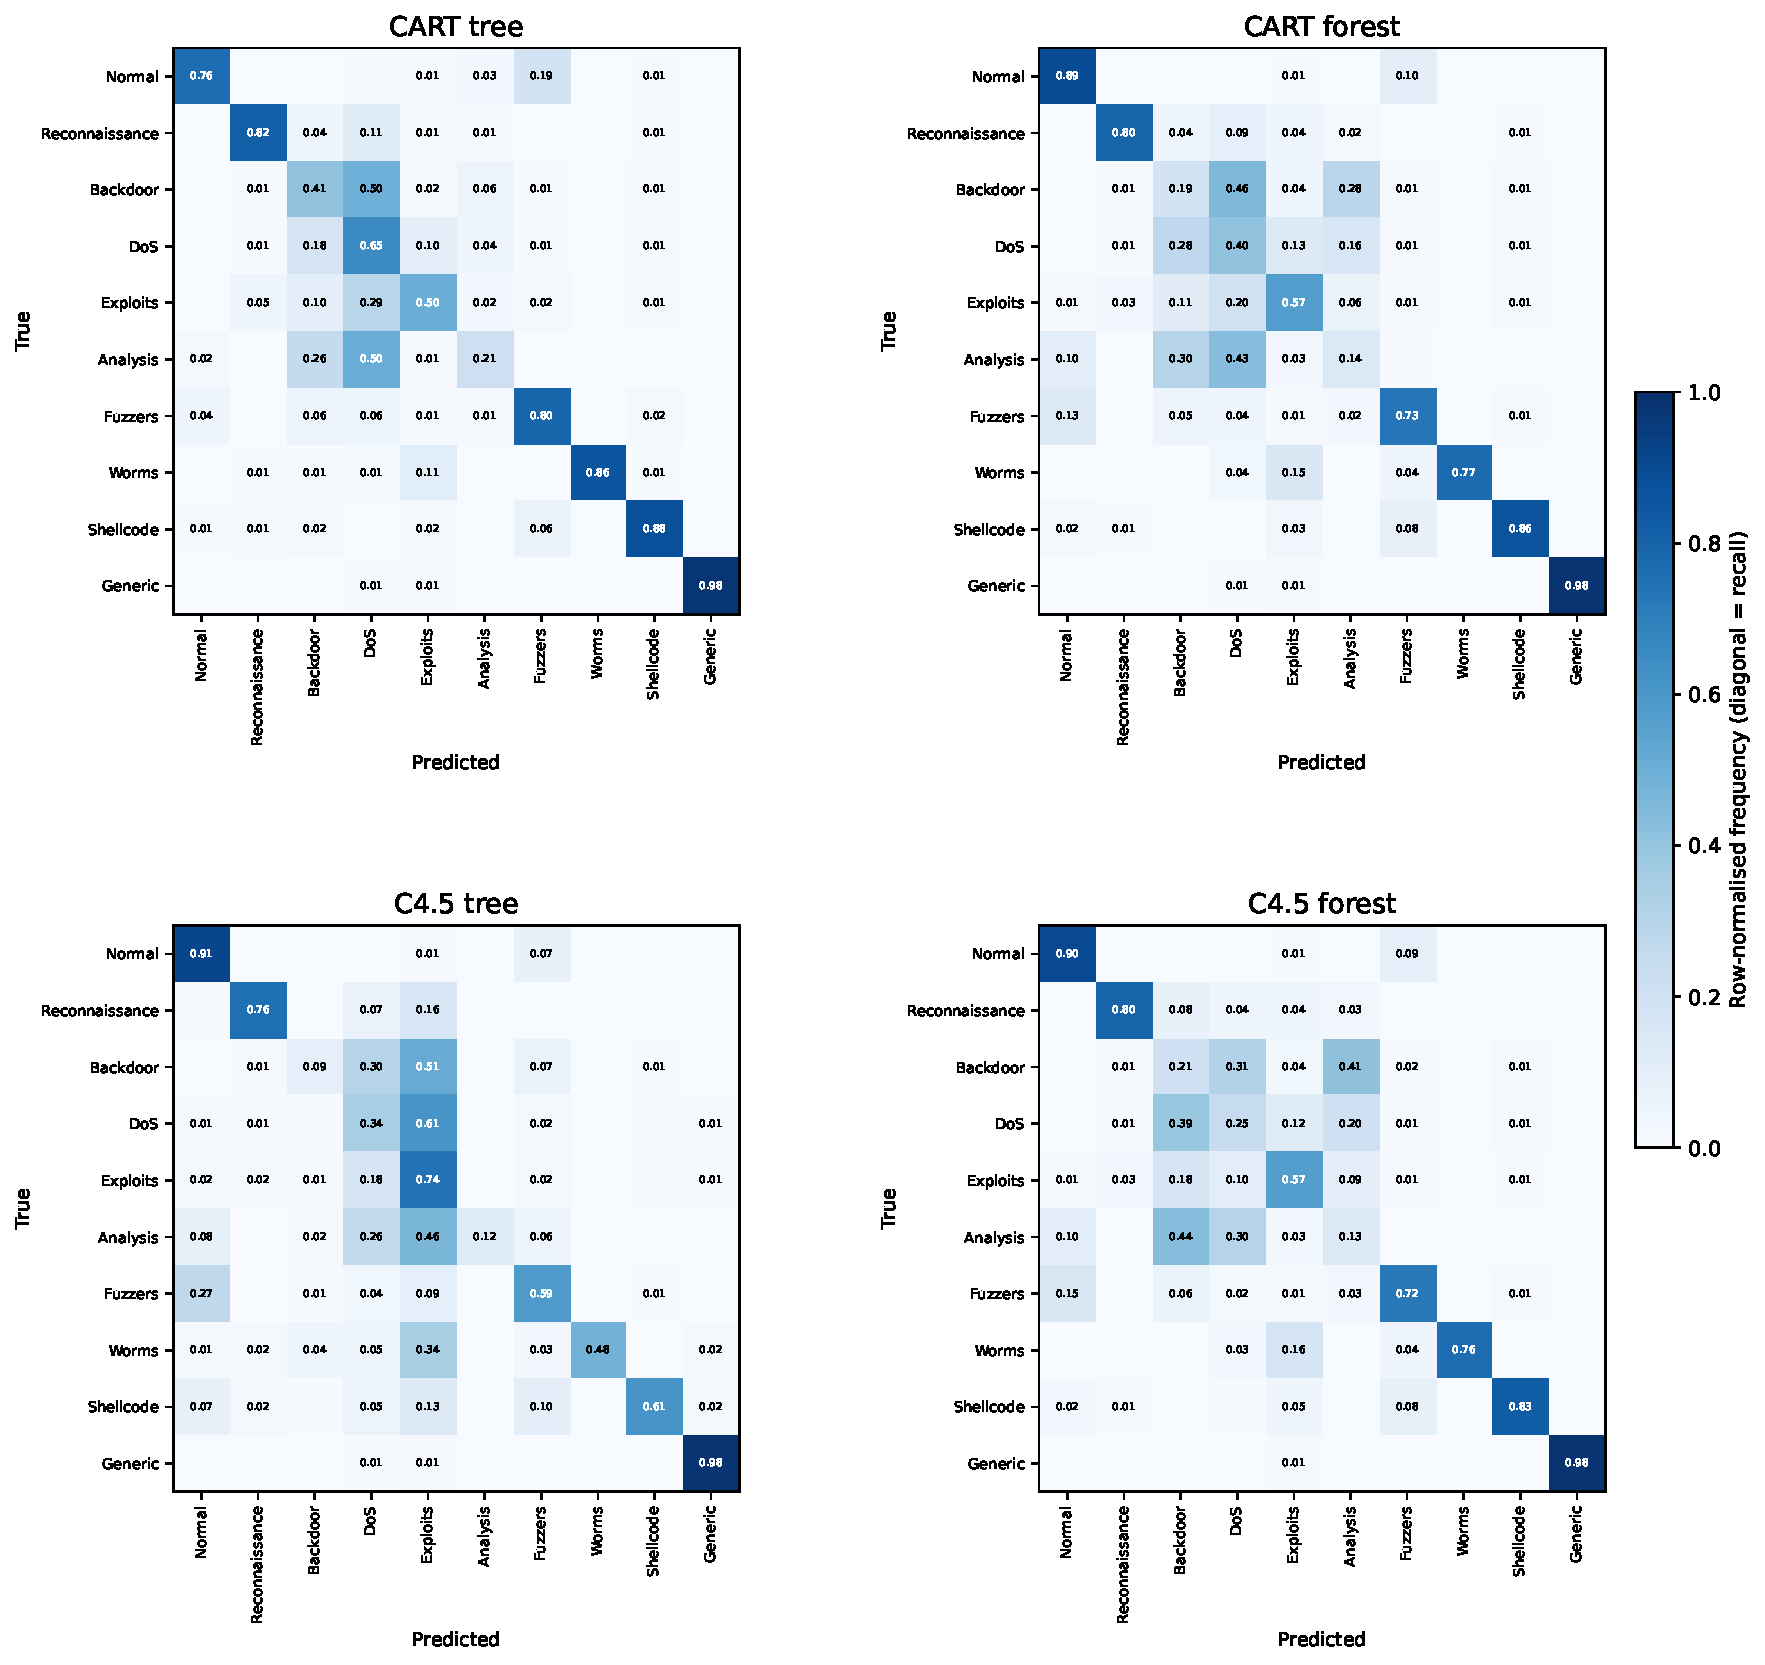
\includegraphics[width=\textwidth]{confusion_matrices.pdf}}{%
\fbox{\parbox{0.6\textwidth}{\centering\vspace{2em} Confusion-matrix figure placeholder ---
generate \texttt{confusion\_matrices.pdf} from the notebook.\vspace{2em}}}}
\caption{Row-normalised confusion matrices for the four tree-based models on the training/test set.
Each row gives the distribution of predictions for a true class, so the diagonal is that class's
recall. Rows are far more informative than raw counts under the severe class imbalance.}
\label{fig:confusion}
\end{figure*}

Table~\ref{tab:results} shows the macro-$F_1$ and overall accuracy of the four tree-based models on the
training/test set, and Figure~\ref{fig:confusion} shows the corresponding per-class behaviour. All
four comfortably outperform the kNN baseline model of the prior work ($0.548$), in line with the Background's
argument that a model partitioning on individual features suits this mixed numeric--nominal,
imbalanced data better than a distance-based one. The focus here is therefore on the differences
among the tree-based models themselves. From the results, a few observations stand out.

Ensembling improved both base learners, but by a small margin. The CART forest improves on
the CART tree ($0.580 \to 0.588$), and the C4.5 forest on the C4.5 tree ($0.577 \to 0.586$), gains
of around $0.008$ in each case. Though there is consistency in the direction of improvement, the size
is very modest. Given that the per-fold standard deviations (Table~\ref{tab:results}) lie between $0.007$ and $0.010$, this means each
ensembling gain is on the order of a single standard deviation. Bagging therefore helps, as the
bias--variance argument stated earlier predicts, but the effect on this dataset is slight rather than dramatic.

The other main finding, likely the most valuable, is that the choice of base learner makes almost no difference. CART and C4.5
are separated by at most $0.003$ in macro-$F_1$ both as single trees ($0.580$ versus $0.577$) and as
forests ($0.588$ versus $0.586$) --- differences well within the fold-to-fold variation and
therefore not really meaningful. The theorised advantages of C4.5, namely multi-way categorical splits and
gain ratio, do not translate into improved performance here. This is consistent with the tuning
result that plain information gain was selected over gain ratio for both C4.5 models: the
high-cardinality features that gain ratio is designed to discount are genuinely informative on this
data, so correcting for the many-valued bias is unnecessary. The best-performing model overall is
the CART forest at $0.588$, but it is effectively tied with the C4.5 forest at $0.586$.

In answer to the question posed in the Background --- whether performance could be improved by using
a different tree or by aggregating trees into an ensemble --- ensembling yields a small but
consistent gain, whereas switching the base learner from CART to C4.5 does not. The best model
improves on the Assignment~2 classification tree ($0.580 \to 0.588$), again only marginally.

The earlier mentioned expectation that forest performance is insensitive to the number of trees beyond
a point was also confirmed. For both forests, increasing the number of trees from $100$ to $300$
changed the macro-$F_1$ by less than the fold-to-fold standard deviation, indicating that
performance had already plateaued by $100$ trees. Both forests were evaluated with their tuned value
of $300$ trees, though the plateau means $100$ would have sufficed.

\begin{table}[t]
\centering
\footnotesize
\setlength{\tabcolsep}{4pt}
\caption{Per-class $F_1$ on the training/test set (pooled out-of-fold predictions). The large classes
are handled well by every model. The models differ mainly on the minority classes (in bold: \texttt{Backdoor},
\texttt{Analysis}, \texttt{Shellcode} and \texttt{Worms}) and on the confusable \texttt{DoS}. The
bottom row is the macro-average reported in Table~\ref{tab:results}.}
\label{tab:perclassf1}
\begin{tabular}{lcccc}
\toprule
Class & \shortstack{CART\\tree} & \shortstack{C4.5\\tree} & \shortstack{CART\\forest} & \shortstack{C4.5\\forest} \\
\midrule
Normal         & 0.86 & 0.92 & 0.92 & 0.92 \\
Reconnaissance & 0.82 & 0.82 & 0.84 & 0.84 \\
\textbf{Backdoor}       & 0.14 & 0.14 & 0.06 & 0.05 \\
DoS            & 0.46 & 0.33 & 0.36 & 0.29 \\
Exploits       & 0.64 & 0.69 & 0.68 & 0.68 \\
\textbf{Analysis}       & 0.15 & 0.19 & 0.07 & 0.06 \\
Fuzzers        & 0.62 & 0.61 & 0.68 & 0.68 \\
\textbf{Worms}          & 0.59 & 0.49 & 0.65 & 0.70 \\
\textbf{Shellcode}      & 0.54 & 0.60 & 0.62 & 0.65 \\
Generic        & 0.99 & 0.99 & 0.99 & 0.99 \\
\midrule
Macro average  & 0.580 & 0.577 & 0.588 & 0.586 \\
\bottomrule
\end{tabular}
\end{table}

Because macro-$F_1$ weights every class equally, the lowest-scoring classes drag it down as much as
the highest-scoring ones lift it, so its value is held back by the hardest classes. The largest class, \texttt{Generic}, is classified almost perfectly by every model
($F_1 \approx 0.99$). \texttt{Normal} is also classified well overall, but Figure~\ref{fig:confusion}
shows that it is consistently confused with \texttt{Fuzzers}, which lowers its recall to between
$0.76$ and $0.91$. The score is held down more severely by the hardest classes (Table~\ref{tab:perclassf1}),
primarily \texttt{Backdoor}, \texttt{Analysis} and \texttt{DoS}. Of these, only \texttt{Backdoor}
and \texttt{Analysis} are genuine minorities, whereas \texttt{DoS} is a mid-sized class whose low
$F_1$ comes from confusion with other classes rather than rarity. The effect of class
weighting can be seen in the per-class breakdown: the balanced-weighted forests achieve notably higher
\emph{recall} on the rarest classes --- the CART forest reaches a recall of $0.77$ on \texttt{Worms}
and $0.86$ on \texttt{Shellcode} --- but at the cost of very low \emph{precision} on \texttt{Backdoor}
and \texttt{Analysis} ($\approx 0.03$--$0.05$), as many instances of other classes are assigned these
minority labels. The unweighted C4.5 tree shows the opposite, with higher precision but much
lower recall on the same classes. Figure~\ref{fig:confusion} shows that these errors are not random:
\texttt{Backdoor}, \texttt{Analysis} and \texttt{DoS} are predominantly confused with one another and
with \texttt{Exploits}, which may point to a genuine overlap between these attack categories rather
than a failure to separate clearly distinct groups. Notably, the rarest class, \texttt{Worms}
($174$ observations), is \emph{not} among the worst performers, indicating that it is the overlap
between classes in the feature space, rather than rarity alone, that drives the remaining errors.

Note that the accuracy column is included only for context and is not used to rank the models, for the
reasons given in the Performance Metric section. 
The accuracy figures nonetheless reinforce the point: the single C4.5 tree achieves the highest accuracy ($0.807$),
but not the best macro-$F_1$, precisely because it is the only model that does not use class weighting
and therefore favours the majority classes. 
Figure~\ref{fig:confusion} further illustrates the trade-off as it can be seen that the balanced-weighted
models forfeit accuracy primarily by assigning a substantial fraction of the large \texttt{Normal}
class to \texttt{Fuzzers} (roughly one in five for the CART tree), an error the unweighted C4.5 tree
mostly avoids. Ranking by accuracy would reward exactly the majority-class bias that this problem
seeks to avoid and would not be appropriate since it isn't the metric that was optimised for.

\section{Conclusion} %[DONE]
% rubric: Conclusions (4)

This work investigated whether the tree-based classifier that performed best in the prior study
could be improved upon, either by replacing CART with a C4.5 base learner or by aggregating trees
into a random forest, comparing all four combinations of the two base learners and the two model
forms on the UNSW-NB15 dataset under a shared macro-$F_1$ protocol.

It was found that ensembling helped, but only marginally with both forests improving on
their respective single trees by roughly $0.008$ in macro-$F_1$.
The CART forest was the best model overall at $0.588$, narrowly ahead
of the Assignment~2 classification tree ($0.580$). The other finding was that the choice of base learner made no
meaningful difference: CART and C4.5 were statistically indistinguishable both as trees and as
forests, and C4.5's theorised advantages, in particular gain ratio, did not materialise, because
the high-cardinality features it discounts turned out to be genuinely informative on this data.

The remaining performance ceiling is set not by the model family but by the data: the minority
attack categories \texttt{Backdoor} and \texttt{Analysis} are intrinsically confused with
\texttt{DoS} and \texttt{Exploits}, so further gains are unlikely to come from refining the tree
algorithm. Future work could instead target this directly, through cost-sensitive or boosting-based
ensembles paired with noise-robust handling, or through feature engineering aimed at separating the
overlapping attack types, rather than through further changes to the base learner.

\nocite{ieeetemplate}
\bibliographystyle{IEEEtran}
\bibliography{references}
% rubric: References (4)

\end{document}
